\begin{frame}
%
\begin{figure}[h]
  \psfrag{cP1}{$\mathcal{P}_1$}
  \psfrag{cP2}{$\mathcal{P}_2$}
  \psfrag{L1}{$L_1$}
  \psfrag{L2}{$L_2$}
  \psfrag{L}{$L$}  
  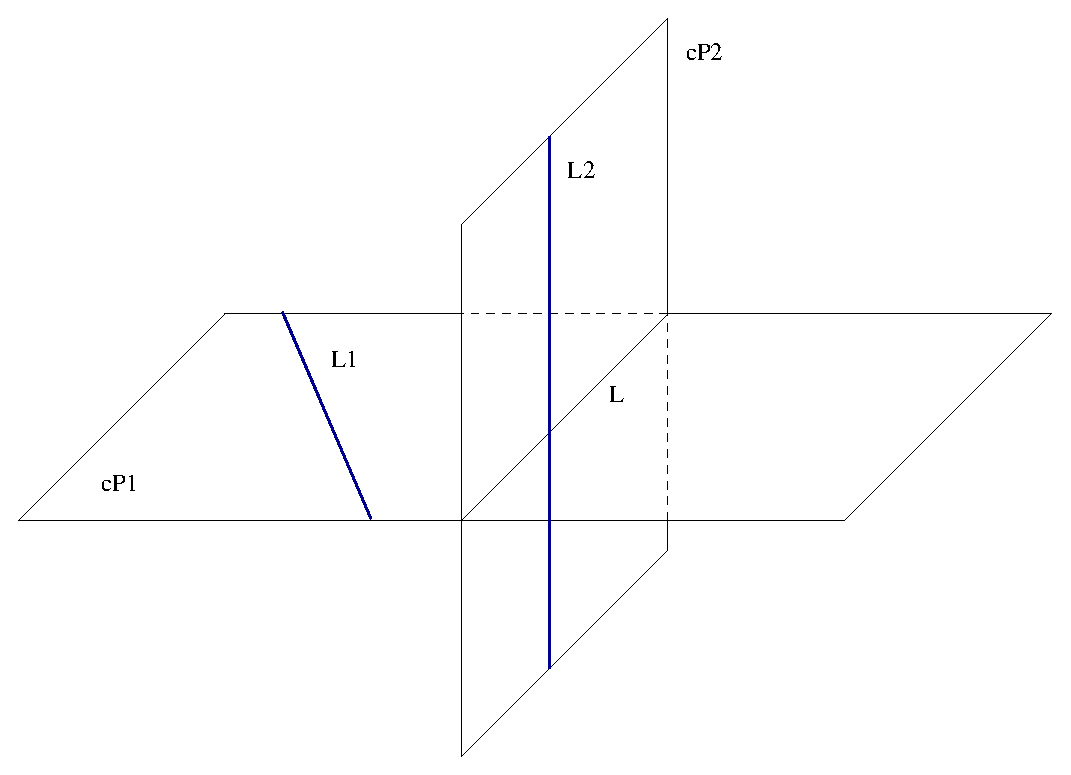
\includegraphics[height=2in]{./images/perpendicularity.eps}
  %\caption{Perpendicularity}
  \label{fig:perpendicularity}
\end{figure}
%
\begin{itemize}
%
\item The planes $\mathcal{P}_1$ and $\mathcal{P}_2$ are perpendicular on each other;
%
\item The lines $L_2$ and $L$ are coplanar and perpendicular on each other;
%
\item The lines $L_1$ and $L_2$ are skew but perpendicular on each other;
%
\item The lines $L_1$ and $L$ are coplanar and not perpendicular;
%
\item The line $L_2$ is perpendicular to the plane $\mathcal{P}_1$;
%
\item The line $L_1$ is not perpendicular to the plane $\mathcal{P}_2$.
\end{itemize}

\end{frame}